%%
%% This is file `acmlarge.tex',
%% generated with the docstrip utility.
%%
%% The original source files were:
%%
%% samples.dtx  (with options: `all,acmlarge')
%% 
%% IMPORTANT NOTICE:
%% 
%% For the copyright see the source file.
%% 
%% Any modified versions of this file must be renamed
%% with new filenames distinct from acmlarge.tex.
%% 
%% For distribution of the original source see the terms
%% for copying and modification in the file samples.dtx.
%% 
%% This generated file may be distributed as long as the
%% original source files, as listed above, are part of the
%% same distribution. (The sources need not necessarily be
%% in the same archive or directory.)
%%
%%
%% Commands for TeXCount
%TC:macro \cite [option:text,text]
%TC:macro \citep [option:text,text]
%TC:macro \citet [option:text,text]
%TC:envir table 0 1
%TC:envir table* 0 1
%TC:envir tabular [ignore] word
%TC:envir displaymath 0 word
%TC:envir math 0 word
%TC:envir comment 0 0
%%
%% The first command in your LaTeX source must be the \documentclass
%% command.
%%
%% For submission and review of your manuscript please change the
%% command to \documentclass[manuscript, screen, review]{acmart}.
%%
%% When submitting camera ready or to TAPS, please change the command
%% to \documentclass[sigconf]{acmart} or whichever template is required
%% for your publication.
%%
%%
\documentclass[acmlarge]{acmart}
%%
%% \BibTeX command to typeset BibTeX logo in the docs
\AtBeginDocument{%
  \providecommand\BibTeX{{%
    Bib\TeX}}}

%% Rights management information.  This information is sent to you
%% when you complete the rights form.  These commands have SAMPLE
%% values in them; it is your responsibility as an author to replace
%% the commands and values with those provided to you when you
%% complete the rights form.
\setcopyright{acmlicensed}
%\copyrightyear{2026}
%\acmYear{2026}
%\acmDOI{XXXXXXX.XXXXXXX}

%% These commands are for a JOURNAL article.
%\acmJournal{POMACS}
%\acmVolume{X}
%\acmNumber{X}
%\acmArticle{XXX}
%\acmMonth{X}

%%
%% Submission ID.
%% Use this when submitting an article to a sponsored event. You'll
%% receive a unique submission ID from the organizers
%% of the event, and this ID should be used as the parameter to this command.
%%\acmSubmissionID{123-A56-BU3}

%%
%% For managing citations, it is recommended to use bibliography
%% files in BibTeX format.
%%
%% You can then either use BibTeX with the ACM-Reference-Format style,
%% or BibLaTeX with the acmnumeric or acmauthoryear sytles, that include
%% support for advanced citation of software artefact from the
%% biblatex-software package, also separately available on CTAN.
%%
%% Look at the sample-*-biblatex.tex files for templates showcasing
%% the biblatex styles.
%%
%%
%% The majority of ACM publications use numbered citations and
%% references.  The command \citestyle{authoryear} switches to the
%% "author year" style.
%%
%% If you are preparing content for an event
%% sponsored by ACM SIGGRAPH, you must use the "author year" style of
%% citations and references.
%% Uncommenting
%% the next command will enable that style.
%%\citestyle{acmauthoryear}


%%
%% end of the preamble, start of the body of the document source.

\begin{document}

%%
%% The "title" command has an optional parameter,
%% allowing the author to define a "short title" to be used in page headers.
\title{Junkyard Benchmarking: Assessing Repurposed Smartphone Cluster Performance in Classroom Autograders}

%%
%% The "author" command and its associated commands are used to define
%% the authors and their affiliations.
%% Of note is the shared affiliation of the first two authors, and the
%% "authornote" and "authornotemark" commands
%% used to denote shared contribution to the research.
\author{Abas Mohamed}
\email{aam037@ucsd.edu}
\authornote{All authors contributed equally to this research.}
%%\orcid{1234-5678-9012}
%%\author{G.K.M. Tobin}
%%\correspondingauthor
%%\email{webmaster@marysville-ohio.com}
\affiliation{%
  \institution{University of California, San Diego}
  \city{La Jolla}
  \state{California}
  \country{USA}
}

\author{Ayushmaan Puri}
\authornotemark[1]
\affiliation{%
  \institution{University of California, San Diego}
  \city{La Jolla}
  \state{California}
  \country{USA}}
\email{aypuri@ucsd.edu}

\author{Richard Vo}
\authornotemark[1]
\affiliation{%
  \institution{University of California, San Diego}
  \city{La Jolla}
  \state{California}
  \country{USA}}
\email{rivo@ucsd.edu}

\author{Shuzheng Zhang}
\authornotemark[1]
\orcid{0009-0001-9438-7685}
\affiliation{%
  \institution{University of California, San Diego}
  \city{La Jolla}
  \state{California}
  \country{USA}}
\email{shz078@ucsd.edu}


%%
%% By default, the full list of authors will be used in the page
%% headers. Often, this list is too long, and will overlap
%% other information printed in the page headers. This command allows
%% the author to define a more concise list
%% of authors' names for this purpose.
%\renewcommand{\shortauthors}{Trovato et al.}

%%
%% The abstract is a short summary of the work to be presented in the
%% article.
\begin{abstract}

The Junkyard Project \cite{10.1145/3575693.3575710} aims to repurpose old and unusable smartphones as compute units for distributed computing \cite{switzer2025hardware}. One target use case is academic autograding; in the most recent offering of \textit{Intro to Parallel Computing}, 330 students shared just 40 GPU nodes on DSMLP\footnote{UCSD's Data Science and Machine Learning Platform}, and demand routinely spiked around deadlines. Student submissions don't need raw GPU power; they need a consistent, available execution environment. Repurposed smartphones fit perfectly: power-efficient, self-contained, standardized, and sourceable at near-zero cost. A dedicated phone cluster eliminates competition for shared HPC resources. This project results in a pipeline that will estimate how many phones are needed to serve a class of $n$ students without meaningful queuing delays.

\end{abstract}

\begin{CCSXML}
<ccs2012>
   <concept>
       <concept_id>10010405.10010489.10010490</concept_id>
       <concept_desc>Applied computing~Computer-assisted instruction</concept_desc>
       <concept_significance>500</concept_significance>
       </concept>
   <concept>
       <concept_id>10002944.10011123.10011674</concept_id>
       <concept_desc>General and reference~Performance</concept_desc>
       <concept_significance>500</concept_significance>
       </concept>
   <concept>
       <concept_id>10003033.10003079.10003080</concept_id>
       <concept_desc>Networks~Network performance modeling</concept_desc>
       <concept_significance>300</concept_significance>
       </concept>
   <concept>
       <concept_id>10010405.10010489.10010491</concept_id>
       <concept_desc>Applied computing~Interactive learning environments</concept_desc>
       <concept_significance>300</concept_significance>
       </concept>
   <concept>
       <concept_id>10010147.10010341.10010349.10010360</concept_id>
       <concept_desc>Computing methodologies~Interactive simulation</concept_desc>
       <concept_significance>500</concept_significance>
       </concept>
 </ccs2012>
\end{CCSXML}

\ccsdesc[500]{Applied computing~Computer-assisted instruction}
\ccsdesc[500]{General and reference~Performance}
\ccsdesc[300]{Networks~Network performance modeling}
\ccsdesc[300]{Applied computing~Interactive learning environments}
\ccsdesc[500]{Computing methodologies~Interactive simulation}


%\received{20 February 2007}
%\received[revised]{12 March 2009}
%\received[accepted]{5 June 2009}

%%
%% This command processes the author and affiliation and title
%% information and builds the first part of the formatted document.
\maketitle


\section{Project Introduction}

% ============================================================
%  Introduction section
%  Compile with: pdflatex main && bibtex main && pdflatex main (x2)
%  Requires: \bibliographystyle{ACM-Reference-Format}
%            \bibliography{references}
%  at the end of your main document.
% ============================================================

Modern computer science education increasingly depends on shared
high-performance computing (HPC) infrastructure. Universities pool GPU
and CPU resources into shared clusters, giving students access to
hardware they could not otherwise afford and enabling courses to assign
computationally intensive work at scale. University-operated HPC
systems are, however, significantly under-resourced relative to
industry and national laboratories~\cite{hpcsurvey2025}, and during
peak demand researchers and students alike face long wait times that
slow iteration-heavy workflows~\cite{hpcsurvey2025}. These pressures
are most acute in instructional settings, where deadline-driven
submission patterns cause demand to spike sharply and unpredictably.

In a recent offering of Intro to Parallel Computing at UC San Diego,
330 students shared just 40 reservable GPU nodes on the campus DSMLP
cluster. During low-traffic periods the allocation was adequate.
Around assignment deadlines, queues grew long enough to delay feedback
by hours. This reflects a broader structural mismatch between
shared, general-purpose compute and the highly variable demand
patterns of large programming courses.

Automated grading systems---autograders---are now a standard tool for
managing courses at this scale. They provide immediate, consistent
feedback without requiring large instructional teams, and make it
practical to run larger courses~\cite{keuning2018}. More frequent
engagement with autograder feedback is also associated with improved
student outcomes~\cite{tran2025}. But autograders are only as
effective as the infrastructure running them. If the execution
environment is shared with other workloads, availability becomes inconsistent, and the feedback loop breaks down precisely when students need it most.

Critically, student submissions for an introductory parallel computing
course do not require high-end GPU throughput. They need a standardized
execution environment that returns consistent, reproducible results
quickly. A cluster of repurposed smartphones can provide exactly this,
at a fraction of the cost of purpose-built server hardware and without
competing for shared HPC allocations.

The case for smartphone-based clusters is well established in prior work. Ranganathan et al.\ demonstrated the feasibility of running automated academic grading on a repurposed phone cluster, showing that even a four-phone cluster can process 33 grading tasks per minute~\cite{ranganathan2025junkyard}. Switzer et al.\ showed more broadly that such clusters are between 9.8$\times$ and 18.9$\times$ more carbon efficient than equivalent cloud instances~\cite{10.1145/3575693.3575710}. Ngoy et al.\ further showed that e-waste smartphones can be repurposed as small-scale data centers capable of efficiently processing and storing data~\cite{ngoy2025ewaste}. Beyond computational performance, the environmental case is compelling on its own: the WEEE Forum and UNITAR estimate that in 2022 alone, roughly 5.3 billion mobile phones were discarded globally, the vast majority destined for landfills or incineration despite remaining functionally intact~\cite{weeeforum2022}. Redirecting even a small fraction of these devices into educational infrastructure extends their useful life and offsets demand for newly manufactured hardware.

Smartphones are not without challenges as compute nodes. They are designed for battery-operated consumer use, and their aggressive power governors throttle CPU and GPU frequency under sustained load, making consistent performance harder to fully guarantee. Flashing a standard Linux distribution to replace the stock OS is a prerequisite for cluster-grade control, and the process is device-specific and labor-intensive. That said, their standardized hardware profiles make execution environments reproduible across nodes once deployed, and their ubiquity means institutions can source them at little to no cost. For the autograding use case specifically, were worloads are short-lived and latency tolerance is moderate, these tradeoffs are acceptable. A dedicated phone cluster still offers a meaningfull improvement over competing for slots on an oversubscribed shared HPC system.

This paper investigates how many phones are needed to serve a class of $n$ students without meaningful queuing delays, and presents a principled estimation strategy grounded in real submission data from a recent course offering.

\section{Related Works}
 
\subsection{Smartphone Repurposing for Distributed Computing}
 
The idea of repurposing consumer mobile hardware as distributed compute
nodes has gained traction as smartphone performance has grown faster
than device replacement cycles. Early work established basic
feasibility: Büsching et al.\ built a six-node Android cluster running
LINPACK benchmarks via MPI, demonstrating that smartphone compute
capacity is comparable to workstation-class hardware of the same
era~\cite{busching2012droidcluster}. Arslan et al.\ developed CWC
(Computing with Charging), a scheduling framework for distributed
smartphone tasks that achieved 1.6$\times$ faster task completion than
baseline approaches by exploiting charging idle time~\cite{arslan2015cwc}.
Sanches proposed a framework for processing batch and streaming data on
mobile device clouds using a move-computation-to-data strategy to
reduce inter-device data exchange~\cite{sanches2017distributed}.
 
These early systems, however, used temporarily idle devices rather than
dedicated repurposed hardware. Switzer et al.\ addressed this
distinction directly by building a cloudlet of repurposed Pixel~3A
phones and introducing the Computational Carbon Intensity (CCI) metric,
which quantifies the carbon efficiency of extending a device's useful
life relative to manufacturing a replacement. Their results showed
smartphone clusters to be 9.8$\times$--18.9$\times$ more carbon
efficient than equivalent AWS EC2 instances across several
microservice workloads~\cite{10.1145/3575693.3575710}. Switzer's
subsequent dissertation extended this analysis to a broader class of
repurposed hardware and formalized the hardware repurposing design
space~\cite{switzer2025hardware}. Ranganathan et al.\ built directly on
this platform, deploying Kubernetes and Docker on a 16-phone cluster of
Google Pixel Fold devices to support both serverless autograding and
distributed computer vision inference~\cite{ranganathan2025junkyard}.
Ngoy et al.\ independently demonstrated repurposed e-waste smartphones
as small-scale data centers for sensor data processing, with
reprogrammability achievable at approximately 8\euro{} per
device~\cite{ngoy2025ewaste}.
 
A parallel line of work has characterized the software challenges of
heterogeneous smartphone clusters. Du et al.\ introduced Molecule, the
first serverless computing system designed for heterogeneous hardware,
achieving higher function density and lower latency than
homogeneous-only systems~\cite{du2022molecule}. Von Leon et al.\
demonstrated that containerized workloads can run successfully on
distributed clusters of low-power edge devices, establishing the
container-as-abstraction model that later phone cluster work
inherits~\cite{vonleon2018container}. Ward and Gittens proposed
frameworks for systematically assessing and cataloguing retired phones
for reuse, addressing the practical challenge that decommissioned
devices exist in varied states of functionality~\cite{ward2018repurposing}.
 
\subsection{Autograding Infrastructure}
 
Automated grading systems have become standard in large programming
courses. Keuning et al.\ conducted a systematic literature review of
101 autograding tools, finding that most provide fully automated
assessment with near-instantaneous feedback and support for multiple
resubmissions~\cite{keuning2018}. Their review established that
immediate feedback and consistent evaluation criteria are the primary
drivers of student satisfaction and learning outcomes. Zhang et al.\
extended this empirical picture with an observational study across five
community colleges, finding that students who check autograder feedback
more frequently achieve measurably higher scores~\cite{tran2025}.
 
The infrastructure behind autograders has received less attention than
the grading logic itself. Gradescope, the platform used in this work,
executes each student submission in a dedicated Ubuntu-based EC2
instance provisioned through AWS~\cite{ranganathan2025junkyard}. While
this provides strong isolation and consistency, it means every
submission consumes cloud compute regardless of workload complexity.
For large courses with hundreds of concurrent submissions around
deadlines, this architecture contributes to the very resource
contention it aims to abstract away from. The GreenGrader system of
Ranganathan et al.\ demonstrated that the grading computation itself
can be offloaded to a phone cluster while remaining compatible with
Gradescope's execution model, achieving a throughput of 33 grading
tasks per minute on a four-phone cluster~\cite{ranganathan2025junkyard}.
 
\subsection{Shared HPC in Academic Settings}
 
University-operated HPC systems are a critical resource for both
research and instruction, but they remain significantly
under-resourced relative to industry and national laboratory
infrastructure~\cite{hpcsurvey2025}. Institutions such as Stanford,
Columbia, and Georgia Tech maintain shared clusters specifically for
coursework, but allocations are fixed and usage is governed by
policies designed primarily around research workloads rather than the
bursty, deadline-driven patterns of student
submissions~\cite{hpcsurvey2025}. This mismatch is well documented: shared
clusters experience long wait times and degraded throughput precisely
during peak instructional demand~\cite{hpcsurvey2025}. Proposals to
address this have included cloud bursting, priority-based scheduling,
and dedicated instructional partitions, but each introduces either
cost, complexity, or fairness tradeoffs that are difficult to resolve
within a course budget.
 
\subsection{Sustainable Computing and E-Waste}
 
The environmental motivation for hardware repurposing is grounded in
manufacturing carbon, not operational energy. Suckling and Lee's life
cycle analysis of smartphones found that manufacturing dominates
greenhouse gas emissions over the device lifetime, meaning that
extending device life through repurposing yields a substantially better
carbon outcome than recycling or disposal~\cite{suckling2015lifecycle}.
The scale of the problem is significant: the WEEE Forum and UNITAR
estimate that 5.3 billion mobile phones were discarded in 2022 alone,
forming a major fraction of the 62 million tonnes of global e-waste
generated that year~\cite{weeeforum2022}. Despite containing valuable
metals and largely functional compute hardware, the majority of these
devices are hoarded, landfilled, or incinerated. Repurposing programs
that redirect even a small fraction of this stock into productive use
extend device lifetimes, displace new hardware manufacturing, and
reduce the total embodied carbon of a computing deployment.
 

\section{Project Overview}

\begin{figure}[h]
  \centering
 
\includegraphics[width=1\linewidth]{final/images/workflow_updated.png}
  \caption{Project Workflow}
  \Description{Project Workflow}
  \label{fig:project_workflow}
\end{figure}

\section{Historic Data and Analysis}

\subsection{CSE 160 Data}
\subsubsection{Data collection}
Collecting data from CSE 160 was constrained by two factors: Gradescope (e-grader of choice for this class) does not expose an API for bulk data export, and student submission records are protected under FERPA. One of the members on the team ---Tom--- was a part of the instructional staff for the class and therefore had to manually webscrape each programming assignment and anonymize them for the rest of the team to work with.
\subsubsection{Limitations}
Because data collection relied on webscraping Gradescope, we had access only to formal submission records. Interactive development sessions on DSMLP, accessed directly via SSH and independent of Gradescope, were not captured. This means that the data reflects assignment submission load but not the ambient compute demand students generate while iterating on their code. Additionally, the webscraping process aggregated results across all execution targets into a single export: submission times reflect grading runs across x86 CPU, NVIDIA GTX 1080Ti, Qualcomm Adreno 643, and Google Pixel Fold nodes without distinguishing between them.


\subsection{Analysis and Modeling}
To characterize student workload patterns, we fit two independent
probabilistic models per programming assignment: one capturing when
submissions arrive over the assignment window, and one capturing how
long submitted jobs take to execute. Both models use Gaussian Mixture
Models (GMMs) selected via the Bayesian Information Criterion (BIC).
All models are fit per assignment.
\subsubsection{Submission Timing Model}
 
Submission timing data was available for all programming assignments.
For each assignment, submission timestamps were converted to hours
elapsed since the first recorded submission, producing a non-negative
scalar for each submission. This parameterization anchors all
assignments to a common relative timeline regardless of absolute
calendar date.
 
We fit a GMM to the resulting distribution of submission hours. The
number of components $k$ was selected by minimizing BIC over the range
$k \in [1,\, \lfloor T/24 \rfloor]$, where $T$ is the total
assignment span in hours, bounding the search to at most one component
per day of the assignment window. Each candidate model was initialized
with ten random restarts (\texttt{n\_init=10}) to reduce sensitivity
to local optima, and trained for up to 500 EM iterations with full
covariance. The resulting mixture takes the form
 
\begin{equation}
    f(t) = \sum_{j=1}^{k} w_j \,\mathcal{N}(t \mid \mu_j,\, \sigma_j^2),
    \label{eq:timing_gmm}
\end{equation}
 
\noindent where $t$ is hours since first submission, and $w_j$,
$\mu_j$, $\sigma_j$ are the weight, mean, and standard deviation of
component $j$, respectively, sorted chronologically by $\mu_j$.
Components correspond naturally to distinct submission bursts, which
we observe to align with the days preceding the assignment deadline.

\subsubsection{Job Runtime Model}
 
Runtime data was available for programming assignments 3, 4, 5, 7, and
8, which were evaluated on execution time in addition to correctness.
The remaining assignments were graded for correctness only and
produced no timing measurements.
 
Before fitting, submissions were partitioned into three categories.
Pre-execution failures --- submissions where the grading container
failed before any student code ran --- produced no runtime measurement
and were excluded entirely. Timeouts, recorded as $-1$ in the dataset,
represent submissions that either exceeded the grader's kill window or
failed to secure an execution node on DSMLP during the Gradescope
handoff; these were excluded from the GMM fit but their frequency was
tracked separately as a timeout fraction $\phi$ of all executed
submissions. The remaining valid runtimes formed the fitting population.
 
Runtime distributions in this setting are right-skewed and span
several orders of magnitude, reflecting the diversity of student
implementations. We therefore log-transformed valid runtimes prior to
fitting, modeling $\log(\text{runtime}_{\text{ms}})$ as a Gaussian
mixture, which is equivalent to modeling the original runtimes as a
mixture of log-normals. The component count $k$ was again selected by
BIC, with the search range bounded by the assignment duration in days,
and each candidate model trained with ten restarts and full covariance.
The mixture in log-space is
 
\begin{equation}
    g(x) = \sum_{j=1}^{k} w_j {N}(x \mid \mu_j,\, \sigma_j^2),
    \quad x = \log(\text{runtime}_{\text{ms}}),
    \label{eq:runtime_gmm}
\end{equation}
 
\noindent with components sorted by $\mu_j$ in ascending order.
For each component, the median runtime in the original millisecond
scale is recovered as $\exp(\mu_j)$, and the 5th and 95th percentiles
as $\exp(\mu_j \mp 1.645\,\sigma_j)$.
 
The timeout fraction $\phi$ is reported alongside the GMM parameters
for each assignment. Timeouts impose a distinct load pattern from
ordinary jobs: rather than completing and releasing a worker, they hold
a worker thread for the full duration of the grader kill window,
making their contribution to cluster load disproportionate to their
count.
 

\subsection{Submission Generation}
To simulate cluster load without requiring live student traffic, we generate synthetic submission traces by sampling from the fitted GMMs described in the previous section. Each synthetic trace represents a complete assignment submission period for a class of $n$ students. Based on observed behavior in CSE~160, students submit approximately three attempts per assignment on average, so a class of $n$ students produces roughly $3n$ synthetic submissions. For the reference class size of 330 students, this yields approximately 1,000 submissions per assignment.

\subsubsection{Decoupled Timing and Runtime Sources}
The generator accepts independent PA indices for submission timing and job runtime, allowing the two distributions to be drawn from different assignments. This decoupling is useful when runtime data is unavailable for a given assignment --- recall that only PAs 3, 4, 5, 7, and 8 carry runtime measurements --- and when the goal is to stress-test the cluster under timing patterns from one assignment with runtime characteristics from another. Unless otherwise specified, timing and runtime are drawn from the same assignment.

\subsubsection{Sampling Procedure}
 
Both GMMs are refit from the filtered data at generation time using the same BIC procedure described in Section~\ref{sec:gmm}. Submission arrival times are drawn by sampling $N$ points from the timing GMM and clipping to $[0, \infty)$ to eliminate the small probability mass that full-covariance Gaussians near $t = 0$ place on negative values. Job runtimes are drawn by sampling $N$ points from the runtime GMM in log-space and exponentiating, yielding samples from the underlying log-normal mixture:
 
\begin{equation}
    \hat{r}_i = \exp\!\left( z_i \right), \quad z_i \sim \sum_{j=1}^{k} w_j \,\mathcal{N}(\mu_j, \sigma_j^2).
    \label{eq:runtime_sample}
\end{equation}
 
\noindent Runtime samples are rounded to the nearest millisecond. Submission scores and active-submission flags are not modeled parametrically. Instead, they are drawn with replacement from the empirical distributions observed in the timing PA's data, preserving the marginal distributions of both fields without assuming a parametric form.
 
Once all fields are sampled, submissions are sorted in ascending order of arrival time to produce a chronological trace. The output is a flat CSV with one row per synthetic submission, containing the attempt index, hours since first submission, runtime in milliseconds, score, and active flag. This trace serves as the input workload for the cluster capacity simulation described in Section~\ref{sec:Simulator}.


\section{Cluster Metrics}

\subsection{Strategy}

\begin{figure}[h]
  \centering
 
\includegraphics[width=0.8\linewidth]{final/images/CSE_160_Workflow.png}
  \caption{Workflow for the auto-grading process in CSE 160}
  \Description{Workflow for the auto-grading process in CSE 160}
  \label{fig:160_workflow}
\end{figure}

\subsection{Performance Degradation Model}

\section{Student Interactive Development Sessions}

\subsection{Backgrounds}

In a modern university computer science course, a cluster has two primary functions: to support students during development, and to carry out the auto-grading of assignment submissions. We have covered the auto-grading function of the cluster and will now consider its uses when supporting student development. 

Currently, most computer science courses provide this as a remote session for the students, where students are allocated a virtual machine on a node in the cluster to interact and develop their code. We will refer to this as interactive student development sessions. This is important as it limits the student code to target only the cluster where their code will be graded, providing a consistent environment regardless of the students’ host machine OS and architecture. This is crucial in the case of a parallel computing course like CSE 160, as the students are graded based on their code run-time after applying optimization techniques, and testing on the exact model of GPU is the only way to guarantee passing the requirements for the assignment.

Historically, CSE 160 relied on the DSMLP cluster to provide students with access to Nvidia GeForce GTX 1080 Ti as a reference GPU to test against. However, several factors stemming mainly from a surge of interest in parallel computing now make this approach unviable as class size increases consistently every year \footnote{Data from UCSD evaluation system: Student Evaluation of Teaching (SET)}. As students compete with the auto-grader for GPU allocation, the system collapses. As students find their submissions timing out, they resubmit many times, while also holding on to their allocated GPU for as long as possible, fearing they will not be able to get through the queue before the assignment deadline. This creates a cycle where the pressure on the cluster continuously increases, blocking the operations of the class.

To relief the pressure on DSMLP, CSE 160 introduced development containers that allow students to develop with their personal machines for correctness before testing on DSMLP for timing, however this has a few drawbacks and does not solve the issue. Most notably, this introduced driver differences as Apple has deprecated OpenCL in 2018, and the course staff resorted to using PoCL\footnote{Portable Computing Language} for running on macOS, which has implementation differences, resulting in a student’s code frequently running correctly on their personal machine, but fails to complete in the auto-grader. This further illustrates the importance of a consistent environment with student development sessions, and the necessity of estimating the cluster size needed with a given class size.

To do this, we require data to base our simulator on. Unfortunately, we do not have data on student session usage from DSMLP, and therefore we present a method of generating these sessions from student submission data.

\subsection{Approach}

We observe that humans have the tendency to complete tasks in bursts, which in this course specifically describes that students tend to work on nothing but their homework before making a submission and letting the auto-grader run. Once they have the results, either they continue working to improve upon it or leave it to come back another time. This is important as it gives us a way to extract development activities from the students from submissions alone.

As an example, Figure~\ref{fig:student_submissions_pa8} is a student’s submission data on PA\footnote{Programming Assignment} 8 in CSE 160. We can see that this student worked on the assignment on March 10th and made two submissions, before pausing and resuming the next day as there is a clear gap between the submissions. The student’s program run-time and score also generally improves as they spend more time on this assignment.

\begin{figure}[h]
  \centering
 
\includegraphics[width=0.5\linewidth]{images/student-submissions.png}
  \caption{A list of one student's submissions for PA8, CSE 160, Winter 2026}
  \Description{A list of one student's submissions for PA8, CSE 160, Winter 2026.}
  \label{fig:student_submissions_pa8}
\end{figure}

As our Gradescope-scraper retrieves the submission data of a student and logs them together, the output will be in order of their attempt, and so we can then safely assign a mock student ID to the student, forming the basis of our analysis as we now have all submissions made by one student.

This type of event is described in \textit{Measuring and modeling bursty human phenomena} \cite{karsai2024measuringmodelingburstyhuman}, which we will be using as the basis for development sessions. A few approaches to detect a burst were described, however, we will simply detect if a submission is inside of a burst by seeing if $\tau$, the time between submissions, is greater than 3 hours, as we have determined it is very unlikely that a student will be continuously working on an assignment if they make no submissions within 3 hours. 

\begin{figure}[h]
  \centering
 
\includegraphics[width=0.8\linewidth]{images/burst-illustration.png}
  \caption{"Schematic diagrams for bursty time series analysis" by Karsai and Jo, used under 
  \href{https://creativecommons.org/licenses/by/4.0/deed.en}{CC BY 4.0}. Unmodified. \cite{karsai2024measuringmodelingburstyhuman}}
  \Description{Schematic diagrams for bursty time series analysis}
  \label{fig:bursty_schematics}
\end{figure}

As shown in Figure~\ref{fig:bursty_schematics}, the submissions are depicted as vertical lines on the time axis, and a burst of submissions depicted as the blue dotted box of time $\Delta t$ is then assigned to them. We will require the following parameters for our generator, which can be changed from the default by the instructor for the specific course and assignment:

\begin{itemize}
  \item $t_{pre} \in \mathbb{Q}^+$: The expected development time before the first submission, modeled with the default Gaussian distribution of $\bar{x}= 3$ hours, $s =$ 1.0
  \item $\tau_{max} \in \mathbb{Q}^+$: The maximum interval between submissions ($\tau$) to be considered as within a burst
  \item $l \in \mathbb{Q}^+$: Randomized lingering time after last submission, modeled with the default Gaussian distribution of $\bar{x}= 0$ hour, $s =$ 0.1
\end{itemize}

We then go through the student's submissions and group them into bursts by $\tau_{max}$, and we now have the discrete array of burst length $\Delta t[n]$ and session start time $x[n]$. We also have the normally generated $t_{pre}[n]$ and $l[n]$ per session, and after combining the parameters, we get the final development sessions for that student:

$$sessions_{a} = \sum_{i=1}^{n} x[i]-t_{pre}[i], lengths_{a} = \Delta t[i] + l[i]$$

Where $a$ is the specific student, $n$ is the number of sessions, and $i$ is one specific session.

\subsection{Limitations}

However, this strategy is severely limited, as we require historic student data as the basis for session generation, making synthetic data incompatible. Furthermore, because we require submissions from individual students, most students do not make enough submissions so that they are statistically significant, and therefore we cannot model and scale the interactive development sessions. It is also not applicable to assignments where the submissions have a rate limit, as it artificially influences the data. Therefore, we can only use this data in our simulator for a class size of the exact number of students that were in CSE 160.

\section{Simulator}

\section{Results}

\section{Conclusion}

\section{Blah Blah Blah}

\subsection{Template Styles}

The primary parameter given to the ``\verb|acmart|'' document class is
the {\itshape template style} which corresponds to the kind of publication
or SIG publishing the work. This parameter is enclosed in square
brackets and is a part of the {\verb|documentclass|} command:
\begin{verbatim}
  \documentclass[STYLE]{acmart}
\end{verbatim}

Journals use one of three template styles. All but three ACM journals
use the {\verb|acmsmall|} template style:
\begin{itemize}
\item {\texttt{acmsmall}}: The default journal template style.
\item {\texttt{acmlarge}}: Used by JOCCH and TAP.
\item {\texttt{acmtog}}: Used by TOG.
\end{itemize}

The majority of conference proceedings documentation will use the {\verb|acmconf|} template style.
\begin{itemize}
\item {\texttt{sigconf}}: The default proceedings template style.
\item{\texttt{sigchi}}: Used for SIGCHI conference articles.
\item{\texttt{sigplan}}: Used for SIGPLAN conference articles.
\end{itemize}

\subsection{Template Parameters}

In addition to specifying the {\itshape template style} to be used in
formatting your work, there are a number of {\itshape template parameters}
which modify some part of the applied template style. A complete list
of these parameters can be found in the {\itshape \LaTeX\ User's Guide.}

Frequently-used parameters, or combinations of parameters, include:
\begin{itemize}
\item {\texttt{anonymous,review}}: Suitable for a ``double-anonymous''
  conference submission. Anonymizes the work and includes line
  numbers. Use with the \texttt{\string\acmSubmissionID} command to print the
  submission's unique ID on each page of the work.
\item{\texttt{authorversion}}: Produces a version of the work suitable
  for posting by the author.
\item{\texttt{screen}}: Produces colored hyperlinks.
\end{itemize}

This document uses the following string as the first command in the
source file:
\begin{verbatim}
\documentclass[acmlarge]{acmart}
\end{verbatim}

\section{Modifications}

Modifying the template --- including but not limited to: adjusting
margins, typeface sizes, line spacing, paragraph and list definitions,
and the use of the \verb|\vspace| command to manually adjust the
vertical spacing between elements of your work --- is not allowed.

{\bfseries Your document will be returned to you for revision if
  modifications are discovered.}

\section{Typefaces}

The ``\verb|acmart|'' document class requires the use of the
``Libertine'' typeface family. Your \TeX\ installation should include
this set of packages. Please do not substitute other typefaces. The
``\verb|lmodern|'' and ``\verb|ltimes|'' packages should not be used,
as they will override the built-in typeface families.

\section{Title Information}

The title of your work should use capital letters appropriately -
\url{https://capitalizemytitle.com/} has useful rules for
capitalization. Use the {\verb|title|} command to define the title of
your work. If your work has a subtitle, define it with the
{\verb|subtitle|} command.  Do not insert line breaks in your title.

If your title is lengthy, you must define a short version to be used
in the page headers, to prevent overlapping text. The \verb|title|
command has a ``short title'' parameter:
\begin{verbatim}
  \title[short title]{full title}
\end{verbatim}

\section{Authors and Affiliations}

Each author must be defined separately for accurate metadata
identification.  As an exception, multiple authors may share one
affiliation. Authors' names should not be abbreviated; use full first
names wherever possible. Include authors' e-mail addresses whenever
possible.

Grouping authors' names or e-mail addresses, or providing an ``e-mail
alias,'' as shown below, is not acceptable:
\begin{verbatim}
  \author{Brooke Aster, David Mehldau}
  \email{dave,judy,steve@university.edu}
  \email{firstname.lastname@phillips.org}
\end{verbatim}

The \verb|authornote| and \verb|authornotemark| commands allow a note
to apply to multiple authors --- for example, if the first two authors
of an article contributed equally to the work.

If your author list is lengthy, you must define a shortened version of
the list of authors to be used in the page headers, to prevent
overlapping text. The following command should be placed just after
the last \verb|\author{}| definition:
\begin{verbatim}
  \renewcommand{\shortauthors}{McCartney, et al.}
\end{verbatim}
Omitting this command will force the use of a concatenated list of all
of the authors' names, which may result in overlapping text in the
page headers.

The article template's documentation, available at
\url{https://www.acm.org/publications/proceedings-template}, has a
complete explanation of these commands and tips for their effective
use.

Note that authors' addresses are mandatory for journal articles.

\section{Rights Information}

Authors of any work published by ACM will need to complete a rights
form. Depending on the kind of work, and the rights management choice
made by the author, this may be copyright transfer, permission,
license, or an OA (open access) agreement.

Regardless of the rights management choice, the author will receive a
copy of the completed rights form once it has been submitted. This
form contains \LaTeX\ commands that must be copied into the source
document. When the document source is compiled, these commands and
their parameters add formatted text to several areas of the final
document:
\begin{itemize}
\item the ``ACM Reference Format'' text on the first page.
\item the ``rights management'' text on the first page.
\item the conference information in the page header(s).
\end{itemize}

Rights information is unique to the work; if you are preparing several
works for an event, make sure to use the correct set of commands with
each of the works.

The ACM Reference Format text is required for all articles over one
page in length, and is optional for one-page articles (abstracts).

\section{CCS Concepts and User-Defined Keywords}

Two elements of the ``acmart'' document class provide powerful
taxonomic tools for you to help readers find your work in an online
search.

The ACM Computing Classification System ---
\url{https://www.acm.org/publications/class-2012} --- is a set of
classifiers and concepts that describe the computing
discipline. Authors can select entries from this classification
system, via \url{https://dl.acm.org/ccs/ccs.cfm}, and generate the
commands to be included in the \LaTeX\ source.

User-defined keywords are a comma-separated list of words and phrases
of the authors' choosing, providing a more flexible way of describing
the research being presented.

CCS concepts and user-defined keywords are required for for all
articles over two pages in length, and are optional for one- and
two-page articles (or abstracts).

\section{Sectioning Commands}

Your work should use standard \LaTeX\ sectioning commands:
\verb|\section|, \verb|\subsection|, \verb|\subsubsection|,
\verb|\paragraph|, and \verb|\subparagraph|. The sectioning levels up to
\verb|\subsubsection| should be numbered; do not remove the numbering
from the commands.

Simulating a sectioning command by setting the first word or words of
a paragraph in boldface or italicized text is {\bfseries not allowed.}

Below are examples of sectioning commands.

\subsection{Subsection}
\label{sec:subsection}

This is a subsection.

\subsubsection{Subsubsection}
\label{sec:subsubsection}

This is a subsubsection.

\paragraph{Paragraph}

This is a paragraph.

\subparagraph{Subparagraph}

This is a subparagraph.

\section{Tables}

The ``\verb|acmart|'' document class includes the ``\verb|booktabs|''
package --- \url{https://ctan.org/pkg/booktabs} --- for preparing
high-quality tables.

Table captions are placed {\itshape above} the table.

Because tables cannot be split across pages, the best placement for
them is typically the top of the page nearest their initial cite.  To
ensure this proper ``floating'' placement of tables, use the
environment \textbf{table} to enclose the table's contents and the
table caption.  The contents of the table itself must go in the
\textbf{tabular} environment, to be aligned properly in rows and
columns, with the desired horizontal and vertical rules.  Again,
detailed instructions on \textbf{tabular} material are found in the
\textit{\LaTeX\ User's Guide}.

Immediately following this sentence is the point at which
Table~\ref{tab:freq} is included in the input file; compare the
placement of the table here with the table in the printed output of
this document.

\begin{table}
  \caption{Frequency of Special Characters}
  \label{tab:freq}
  \begin{tabular}{ccl}
    \toprule
    Non-English or Math&Frequency&Comments\\
    \midrule
    \O & 1 in 1,000& For Swedish names\\
    $\pi$ & 1 in 5& Common in math\\
    \$ & 4 in 5 & Used in business\\
    $\Psi^2_1$ & 1 in 40,000& Unexplained usage\\
  \bottomrule
\end{tabular}
\end{table}

To set a wider table, which takes up the whole width of the page's
live area, use the environment \textbf{table*} to enclose the table's
contents and the table caption.  As with a single-column table, this
wide table will ``float'' to a location deemed more
desirable. Immediately following this sentence is the point at which
Table~\ref{tab:commands} is included in the input file; again, it is
instructive to compare the placement of the table here with the table
in the printed output of this document.

\begin{table*}
  \caption{Some Typical Commands}
  \label{tab:commands}
  \begin{tabular}{ccl}
    \toprule
    Command &A Number & Comments\\
    \midrule
    \texttt{{\char'134}author} & 100& Author \\
    \texttt{{\char'134}table}& 300 & For tables\\
    \texttt{{\char'134}table*}& 400& For wider tables\\
    \bottomrule
  \end{tabular}
\end{table*}

Always use midrule to separate table header rows from data rows, and
use it only for this purpose. This enables assistive technologies to
recognise table headers and support their users in navigating tables
more easily.

\section{Math Equations}
You may want to display math equations in three distinct styles:
inline, numbered or non-numbered display.  Each of the three are
discussed in the next sections.

\subsection{Inline (In-text) Equations}
A formula that appears in the running text is called an inline or
in-text formula.  It is produced by the \textbf{math} environment,
which can be invoked with the usual
\texttt{{\char'134}begin\,\ldots{\char'134}end} construction or with
the short form \texttt{\$\,\ldots\$}. You can use any of the symbols
and structures, from $\alpha$ to $\omega$, available in
\LaTeX~\cite{Lamport:LaTeX}; this section will simply show a few
examples of in-text equations in context. Notice how this equation:
\begin{math}
  \lim_{n\rightarrow \infty}x=0
\end{math},
set here in in-line math style, looks slightly different when
set in display style.  (See next section).

\subsection{Display Equations}
A numbered display equation---one set off by vertical space from the
text and centered horizontally---is produced by the \textbf{equation}
environment. An unnumbered display equation is produced by the
\textbf{displaymath} environment.

Again, in either environment, you can use any of the symbols and
structures available in \LaTeX\@; this section will just give a couple
of examples of display equations in context.  First, consider the
equation, shown as an inline equation above:
\begin{equation}
  \lim_{n\rightarrow \infty}x=0
\end{equation}
Notice how it is formatted somewhat differently in
the \textbf{displaymath}
environment.  Now, we'll enter an unnumbered equation:
\begin{displaymath}
  \sum_{i=0}^{\infty} x + 1
\end{displaymath}
and follow it with another numbered equation:
\begin{equation}
  \sum_{i=0}^{\infty}x_i=\int_{0}^{\pi+2} f
\end{equation}
just to demonstrate \LaTeX's able handling of numbering.

\section{Figures}

The ``\verb|figure|'' environment should be used for figures. One or
more images can be placed within a figure. If your figure contains
third-party material, you must clearly identify it as such, as shown
in the example below.
\begin{figure}[h]
  \centering
 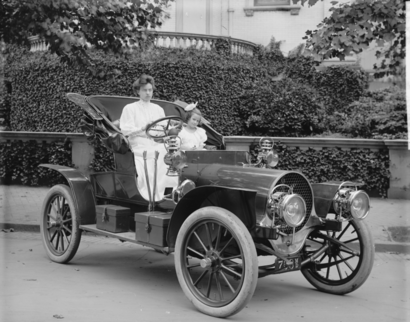
\includegraphics[width=\linewidth]{sample-franklin}
  \caption{1907 Franklin Model D roadster. Photograph by Harris \&
    Ewing, Inc. [Public domain], via Wikimedia
    Commons. (\url{https://goo.gl/VLCRBB}).}
  \Description{A woman and a girl in white dresses sit in an open car.}
\end{figure}

Your figures should contain a caption which describes the figure to
the reader.

Figure captions are placed {\itshape below} the figure.

Every figure should also have a figure description unless it is purely
decorative. These descriptions convey what’s in the image to someone
who cannot see it. They are also used by search engine crawlers for
indexing images, and when images cannot be loaded.

A figure description must be unformatted plain text less than 2000
characters long (including spaces).  {\bfseries Figure descriptions
  should not repeat the figure caption – their purpose is to capture
  important information that is not already provided in the caption or
  the main text of the paper.} For figures that convey important and
complex new information, a short text description may not be
adequate. More complex alternative descriptions can be placed in an
appendix and referenced in a short figure description. For example,
provide a data table capturing the information in a bar chart, or a
structured list representing a graph.  For additional information
regarding how best to write figure descriptions and why doing this is
so important, please see
\url{https://www.acm.org/publications/taps/describing-figures/}.

\subsection{The ``Teaser Figure''}

A ``teaser figure'' is an image, or set of images in one figure, that
are placed after all author and affiliation information, and before
the body of the article, spanning the page. If you wish to have such a
figure in your article, place the command immediately before the
\verb|\maketitle| command:
\begin{verbatim}
  \begin{teaserfigure}
 \includegraphics[width=\textwidth]{sampleteaser}
    \caption{figure caption}
    \Description{figure description}
  \end{teaserfigure}
\end{verbatim}

\section{Citations and Bibliographies}

The use of \BibTeX\ for the preparation and formatting of one's
references is strongly recommended. Authors' names should be complete
--- use full first names (``Donald E. Knuth'') not initials
(``D. E. Knuth'') --- and the salient identifying features of a
reference should be included: title, year, volume, number, pages,
article DOI, etc.

The bibliography is included in your source document with these two
commands, placed just before the \verb|\end{document}| command:
\begin{verbatim}
  \bibliographystyle{ACM-Reference-Format}
  \bibliography{bibfile}
\end{verbatim}
where ``\verb|bibfile|'' is the name, without the ``\verb|.bib|''
suffix, of the \BibTeX\ file.

Citations and references are numbered by default. A small number of
ACM publications have citations and references formatted in the
``author year'' style; for these exceptions, please include this
command in the {\bfseries preamble} (before the command
``\verb|\begin{document}|'') of your \LaTeX\ source:
\begin{verbatim}
  \citestyle{acmauthoryear}
\end{verbatim}


  Some examples.  A paginated journal article \cite{Abril07}, an
  enumerated journal article \cite{Cohen07}, a reference to an entire
  issue \cite{JCohen96}, a monograph (whole book) \cite{Kosiur01}, a
  monograph/whole book in a series (see 2a in spec. document)
  \cite{Harel79}, a divisible-book such as an anthology or compilation
  \cite{Editor00} followed by the same example, however we only output
  the series if the volume number is given \cite{Editor00a} (so
  Editor00a's series should NOT be present since it has no vol. no.),
  a chapter in a divisible book \cite{Spector90}, a chapter in a
  divisible book in a series \cite{Douglass98}, a multi-volume work as
  book \cite{Knuth97}, a couple of articles in a proceedings (of a
  conference, symposium, workshop for example) (paginated proceedings
  article) \cite{Andler79, Hagerup1993}, a proceedings article with
  all possible elements \cite{Smith10}, an example of an enumerated
  proceedings article \cite{VanGundy07}, an informally published work
  \cite{Harel78}, a couple of preprints \cite{Bornmann2019,
    AnzarootPBM14}, a doctoral dissertation \cite{Clarkson85}, a
  master's thesis: \cite{anisi03}, an online document / world wide web
  resource \cite{Thornburg01, Ablamowicz07, Poker06}, a video game
  (Case 1) \cite{Obama08} and (Case 2) \cite{Novak03} and \cite{Lee05}
  and (Case 3) a patent \cite{JoeScientist001}, work accepted for
  publication \cite{rous08}, 'YYYYb'-test for prolific author
  \cite{SaeediMEJ10} and \cite{SaeediJETC10}. Other cites might
  contain 'duplicate' DOI and URLs (some SIAM articles)
  \cite{Kirschmer:2010:AEI:1958016.1958018}. Boris / Barbara Beeton:
  multi-volume works as books \cite{MR781536} and \cite{MR781537}. A
  presentation~\cite{Reiser2014}. An article under
  review~\cite{Baggett2025}. A
  couple of citations with DOIs:
  \cite{2004:ITE:1009386.1010128,Kirschmer:2010:AEI:1958016.1958018}. Online
  citations: \cite{TUGInstmem, Thornburg01, CTANacmart}.
  Artifacts: \cite{R} and \cite{UMassCitations}.

\section{Acknowledgments}

Identification of funding sources and other support, and thanks to
individuals and groups that assisted in the research and the
preparation of the work should be included in an acknowledgment
section, which is placed just before the reference section in your
document.

This section has a special environment:
\begin{verbatim}
  \begin{acks}
  ...
  \end{acks}
\end{verbatim}
so that the information contained therein can be more easily collected
during the article metadata extraction phase, and to ensure
consistency in the spelling of the section heading.

Authors should not prepare this section as a numbered or unnumbered {\verb|\section|}; please use the ``{\verb|acks|}'' environment.

\section{Appendices}

If your work needs an appendix, add it before the
``\verb|\end{document}|'' command at the conclusion of your source
document.

Start the appendix with the ``\verb|appendix|'' command:
\begin{verbatim}
  \appendix
\end{verbatim}
and note that in the appendix, sections are lettered, not
numbered. This document has two appendices, demonstrating the section
and subsection identification method.

\section{Multi-language papers}

Papers may be written in languages other than English or include
titles, subtitles, keywords and abstracts in different languages (as a
rule, a paper in a language other than English should include an
English title and an English abstract).  Use \verb|language=...| for
every language used in the paper.  The last language indicated is the
main language of the paper.  For example, a French paper with
additional titles and abstracts in English and German may start with
the following command
\begin{verbatim}
\documentclass[sigconf, language=english, language=german,
               language=french]{acmart}
\end{verbatim}

The title, subtitle, keywords and abstract will be typeset in the main
language of the paper.  The commands \verb|\translatedXXX|, \verb|XXX|
begin title, subtitle and keywords, can be used to set these elements
in the other languages.  The environment \verb|translatedabstract| is
used to set the translation of the abstract.  These commands and
environment have a mandatory first argument: the language of the
second argument.  See \verb|sample-sigconf-i13n.tex| file for examples
of their usage.

%%
%% The acknowledgments section is defined using the "acks" environment
%% (and NOT an unnumbered section). This ensures the proper
%% identification of the section in the article metadata, and the
%% consistent spelling of the heading.
\begin{acks}
To Robert, for the bagels and explaining CMYK and color spaces.
\end{acks}


\section*{Ethics and Privacy Statement}

This section of your ACM work should discuss the potential societal
risks that might result from its publication; two to three sentences
related to the findings of your study, or new advancements made
possible by their developed methods. The privacy and ethics statement
should clearly address the broader impacts of their work as it relates
to the authors' interpretation of privacy, fairness, safety, human
rights, data sovereignty, or future misuse and any benefit/risk
trade-off resulting from this research. We acknowledge that some
papers may have minimal societal risks beyond those considered by
institutional review boards, and the dimensions considered by any
review of the user study design or dataset licenses could be provided
in this statement.

%%
%% The next two lines define the bibliography style to be used, and
%% the bibliography file.
\bibliographystyle{ACM-Reference-Format}
\bibliography{references}


%%
%% If your work has an appendix, this is the place to put it.
\appendix

\section{Research Methods}

\subsection{Part One}

Lorem ipsum dolor sit amet, consectetur adipiscing elit. Morbi
malesuada, quam in pulvinar varius, metus nunc fermentum urna, id
sollicitudin purus odio sit amet enim. Aliquam ullamcorper eu ipsum
vel mollis. Curabitur quis dictum nisl. Phasellus vel semper risus, et
lacinia dolor. Integer ultricies commodo sem nec semper.

\subsection{Part Two}

Etiam commodo feugiat nisl pulvinar pellentesque. Etiam auctor sodales
ligula, non varius nibh pulvinar semper. Suspendisse nec lectus non
ipsum convallis congue hendrerit vitae sapien. Donec at laoreet
eros. Vivamus non purus placerat, scelerisque diam eu, cursus
ante. Etiam aliquam tortor auctor efficitur mattis.

\section{Online Resources}

Nam id fermentum dui. Suspendisse sagittis tortor a nulla mollis, in
pulvinar ex pretium. Sed interdum orci quis metus euismod, et sagittis
enim maximus. Vestibulum gravida massa ut felis suscipit
congue. Quisque mattis elit a risus ultrices commodo venenatis eget
dui. Etiam sagittis eleifend elementum.

Nam interdum magna at lectus dignissim, ac dignissim lorem
rhoncus. Maecenas eu arcu ac neque placerat aliquam. Nunc pulvinar
massa et mattis lacinia.

\end{document}
\endinput
%%
%% End of file `acmlarge.tex'.
